\documentclass[12pt]{article}

\usepackage{amsthm}
\usepackage{amsmath}
\usepackage{amsfonts}
\usepackage{mathrsfs}
\usepackage{array}
\usepackage{amssymb}
\usepackage{units}
\usepackage{graphicx}
\usepackage{tikz-cd}
\usepackage{nicefrac}
\usepackage{hyperref}
\usepackage{bbm}
\usepackage{color}
\usepackage{tensor}
\usepackage{tipa}
\usepackage{bussproofs}
\usepackage{ stmaryrd }
\usepackage{ textcomp }
\usepackage{leftidx}
\usepackage{afterpage}
\usepackage{varwidth}
\usepackage{tasks}
\usepackage{ cmll }
\usepackage{adjustbox}

\newcommand\blankpage{
	\null
	\thispagestyle{empty}
	\addtocounter{page}{-1}
	\newpage
}

\graphicspath{ {images/} }

\theoremstyle{plain}
\newtheorem{thm}{Theorem}[subsection] % reset theorem numbering for each chapter
\newtheorem{proposition}[thm]{Proposition}
\newtheorem{lemma}[thm]{Lemma}
\newtheorem{fact}[thm]{Fact}
\newtheorem{cor}[thm]{Corollary}

\theoremstyle{definition}
\newtheorem{defn}[thm]{Definition} % definition numbers are dependent on theorem numbers
\newtheorem{exmp}[thm]{Example} % same for example numbers
\newtheorem{notation}[thm]{Notation}
\newtheorem{remark}[thm]{Remark}
\newtheorem{condition}[thm]{Condition}
\newtheorem{question}[thm]{Question}
\newtheorem{construction}[thm]{Construction}
\newtheorem{exercise}[thm]{Exercise}
\newtheorem{example}[thm]{Example}
\newtheorem{aside}[thm]{Aside}

\def\doubleunderline#1{\underline{\underline{#1}}}
\newcommand{\bb}[1]{\mathbb{#1}}
\newcommand{\scr}[1]{\mathscr{#1}}
\newcommand{\call}[1]{\mathcal{#1}}
\newcommand{\psheaf}{\text{\underline{Set}}^{\scr{C}^{\text{op}}}}
\newcommand{\und}[1]{\underline{\hspace{#1 cm}}}
\newcommand{\adj}[1]{\text{\textopencorner}{#1}\text{\textcorner}}
\newcommand{\comment}[1]{}
\newcommand{\lto}{\longrightarrow}
\newcommand{\rone}{(\operatorname{R}\bold{1})}
\newcommand{\lone}{(\operatorname{L}\bold{1})}
\newcommand{\rimp}{(\operatorname{R} \multimap)}
\newcommand{\limp}{(\operatorname{L} \multimap)}
\newcommand{\rtensor}{(\operatorname{R}\otimes)}
\newcommand{\ltensor}{(\operatorname{L}\otimes)}
\newcommand{\rtrue}{(\operatorname{R}\top)}
\newcommand{\rwith}{(\operatorname{R}\&)}
\newcommand{\lwithleft}{(\operatorname{L}\&)_{\operatorname{left}}}
\newcommand{\lwithright}{(\operatorname{L}\&)_{\operatorname{right}}}
\newcommand{\rplusleft}{(\operatorname{R}\oplus)_{\operatorname{left}}}
\newcommand{\rplusright}{(\operatorname{R}\oplus)_{\operatorname{right}}}
\newcommand{\lplus}{(\operatorname{L}\oplus)}
\newcommand{\prom}{(\operatorname{prom})}
\newcommand{\ctr}{(\operatorname{ctr})}
\newcommand{\der}{(\operatorname{der})}
\newcommand{\weak}{(\operatorname{weak})}
\newcommand{\exi}{(\operatorname{exists})}
\newcommand{\fa}{(\operatorname{for\text{ }all})}
\newcommand{\ex}{(\operatorname{ex})}
\newcommand{\cut}{(\operatorname{cut})}
\newcommand{\ax}{(\operatorname{ax})}
\newcommand{\negation}{\sim}
\newcommand{\true}{\top}
\newcommand{\false}{\bot}
\DeclareRobustCommand{\diamondtimes}{%
	\mathbin{\text{\rotatebox[origin=c]{45}{$\boxplus$}}}%
}
\newcommand{\tagarray}{\mbox{}\refstepcounter{equation}$(\theequation)$}
\newcommand{\startproof}[1]{
	\AxiomC{#1}
	\noLine
	\UnaryInfC{$\vdots$}
}
\newenvironment{scprooftree}[1]%
{\gdef\scalefactor{#1}\begin{center}\proofSkipAmount \leavevmode}%
	{\scalebox{\scalefactor}{\DisplayProof}\proofSkipAmount \end{center} }


\title{Category Theory exercise sheet 1}

\begin{document}
	
	\maketitle
	
	\section{Category theory}
	\begin{question}
		What is a category?
		\begin{enumerate}
			\item Pull out a blank sheet of paper and write out the full definition of a category from memory. Once you have finished, check your answer and be scrutinising in your marking (did you write \emph{set} where you shouldn't have? Did you only write \emph{one} sided identities? Did you describe any \emph{data} as a \emph{condition}?)
			
			Redo this exercise every day until you have gotten it absolutely correct three days in a row. Use the following boxes to tick off your progress.
			\begin{center}
				\begin{adjustbox}{width=\columnwidth,center}
			\begin{tabular}{| c | c | c | c | c | c | c |}
				\hline
				\text{Thursday} & \text{Friday} & \text{Saturday} & \text{Sunday} & \text{Monday} & \text{Tuesday} & \text{Wednesday}\\
				\hline
				&&&&&&\\
				\hline
				\end{tabular}
			\end{adjustbox}
			\end{center}
		\item A poset $(P, \leq)$ can be regarded as a category. The objects are the elements of $P$ and there exists a unique morphism $x \lto y$ with domain $x$ and codomain $y$ whenever $x \leq y$. Prove that this is a category.
			\end{enumerate}
		\end{question}
	
	\section{Mathematics}
	\begin{question} We (secretly) investigate \emph{naturality}, a concept which will be defined formally later in the course.
		\begin{enumerate}
			\item\label{basis} Let $V$ be a finite dimensional complex vector space and denote its dual by $V^\ast$. Recall that the underlying set of $V^\ast$ is given by the set of linear functionals with domain $V$ and codomain $\bb{C}$, that is,
			\begin{equation}
				V^\ast := \{ \psi: V \lto \bb{C} \mid \psi\text{ is linear} \}
				\end{equation}
			Fix a basis $\scr{B} = \{ v_1, \ldots, v_n \}$ for $V$. Define the following linear functions.
			\begin{align*}
				v_i^\ast: V &\lto \bb{C}\\
				v &\longmapsto
				\begin{cases}
					1,& v = v_i\\
					0,& v \neq v_i
				\end{cases}
			\end{align*}
		Prove that $\scr{B}$ is a basis for $V^\ast$.
		\item Using part \ref{basis}, prove that the function $\Phi_{V, \scr{B}}: V \lto V^\ast$ defined by linearity along with the following rules
		\begin{align}
			\Phi_{V,\scr{B}}(v_i) = v_i^\ast,\quad \forall i = 1,\ldots, n
			\end{align}
		is an isomorphism.
		\item For any vector $v \in V$ let $\operatorname{Ev}_v: V^\ast \lto \bb{C}$ denote the following function
		\begin{align*}
			\operatorname{Ev}_v: V^\ast &\lto \bb{C}\\
			\psi &\longmapsto \psi(v)
		\end{align*}
		Prove that the following is an isomorphism.
		\begin{align*}
			\Psi_V: V &\lto V^{\ast\ast}\\
			v &\longmapsto \operatorname{Ev}_v
		\end{align*}
		\item Let $\varphi: V \lto W$ be a morphism of finite dimensional vector spaces. Define the following linear function.
		\begin{align*}
			\varphi^\ast: W^\ast &\lto V^\ast\\
			\psi &\longmapsto \psi \circ \varphi
			\end{align*}
		Prove that for any linear transformation $\varphi: V \lto W$ the following diagram commutes.
		\begin{equation}
			\begin{tikzcd}
				V\arrow[r,"{\varphi}"]\arrow[d,swap,"{\Psi_V}"] & W\arrow[d,"{\Psi_W}"]\\
				V^{\ast\ast}\arrow[r,"{\varphi^{\ast\ast}}"] & W^{\ast\ast}
				\end{tikzcd}
			\end{equation}
		That is, prove the following equality of functions.
		\begin{equation}
			\psi_W \circ \varphi = \varphi^{\ast\ast} \circ \Psi_V
			\end{equation}
		\item Find a linear function $\varphi: V \lto W$ for some vector spaces $V,W$ along with choices of bases $\scr{B},\scr{C}$ for $V,W$ respectively such that the following diagram does \emph{not} commute.
		\begin{equation}
			\begin{tikzcd}
			V\arrow[r,"{\varphi}"]\arrow[d,swap,"{\Phi_{V,\scr{B}}}"] & W\arrow[d,"{\Phi_{W, \scr{C}}}"]\\
			V^\ast & W^\ast\arrow[l,"{\varphi^\ast}"]
			\end{tikzcd}
			\end{equation}
			\end{enumerate}
		\end{question}
	
	\section{Computer Science}
	\begin{question}
		A simple system.
		\begin{enumerate}
			\item\label{Hasse} Recall that a relation $R$ on a set $X$ is a subset of the cartesian product $X \times X$. Thus, elements of $R$ consist of pairs $(x_1,x_2)$ of elements in $X$.
			
			Recall also that a relation $R$ is \textbf{transitive} if it satisfies the following property: for all $(x_1,x_2), (x_3, x_4) \in R$ if $x_2 = x_3$ then $(x_1, x_4) \in R$.
			
			If a relation $R$ is not transitive, then we define the \textbf{transitive closure} $\operatorname{T}(R)$ of $R$ to be smallest relation containing $R$ which is transitive. For instance, if $X = \{ x_1, x_2, x_3 \}$ and $R$ is
			\begin{equation}
				R := \{ (x_1, x_2), (x_2, x_3) \}
				\end{equation}
			then
			\begin{equation}
				\operatorname{T}(R) = \{ (x_1, x_2), (x_2, x_3), (x_1, x_3) \} = R \cup \{ (x_1, x_3) \}
				\end{equation}
			Define the \textbf{join} $R_1 \vee R_2$ of two relations $R_1, R_2$ on a set $X$ to be the transitive closure of their union.
			\begin{equation}
				R_1 \vee R_2 := \operatorname{T}(R_1 \cup R_2)
				\end{equation}
			Calculate the join of the following two relations on the implied underlying set with 6 elements.
			\begin{center}
				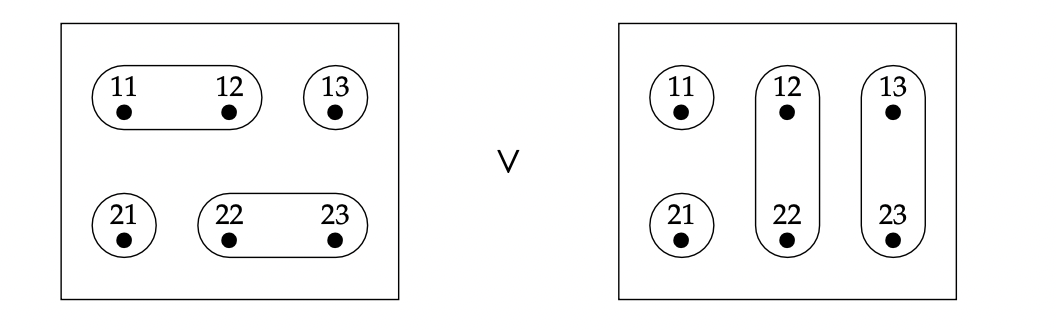
\includegraphics[width=\textwidth]{CompOne.png}
				\end{center}
			\item Given two relations $R_1, R_2$ on a set $X$ we define
			\begin{equation}
				R_1 \leq R_2\text{ if and only if }(x_1, x_2) \in R_1 \Longrightarrow (x_1, x_2) \in R_2
				\end{equation}
			A \textbf{Hasse diagram} is a lattice which shows all the relations along with their inclusions (with respect to $\leq$ just defined). For example, the Hasse diagram of a three element set is given as follows.
			\begin{center}
				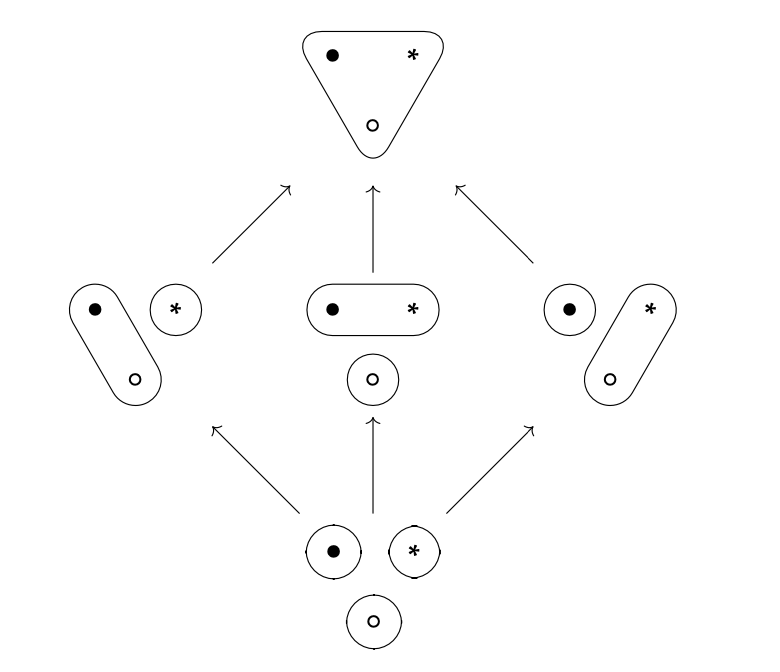
\includegraphics[width=10cm]{CompTwo.png}
			\end{center}
		Write out the Hasse diagram of the four element set $\{ 1,2,3,4 \}$. (How many nodes in your diagram do you expect there to be?)
		\item Choose any two nodes in your Hasse diagram you wrote in \ref{Hasse} and call them $A$ and $B$. Identify $A \vee B$ on your Hasse diagram. Are the following true?
		\begin{equation}
			A \leq A \vee B\qquad B \leq A \vee B
			\end{equation}
		Circle the nodes $C$ for which both $A \leq C$ and $B \leq C$. Is it true that in each case $A \vee B \leq C$?
		
		We will see later that $\vee$ is an example of a \textbf{coproduct}. Another example of a coproduct is the disjoint union $X \coprod Y$ of two sets $X,Y$. We will see later in the course how category theory relates these two concepts.
			\end{enumerate}
		\end{question}
	
	
	
	
	
	
	
	
	
	
	
	
	
	
	
	
	
	
	
	
	
	
	
	
	
	
	
	\end{document}